\begin{figure}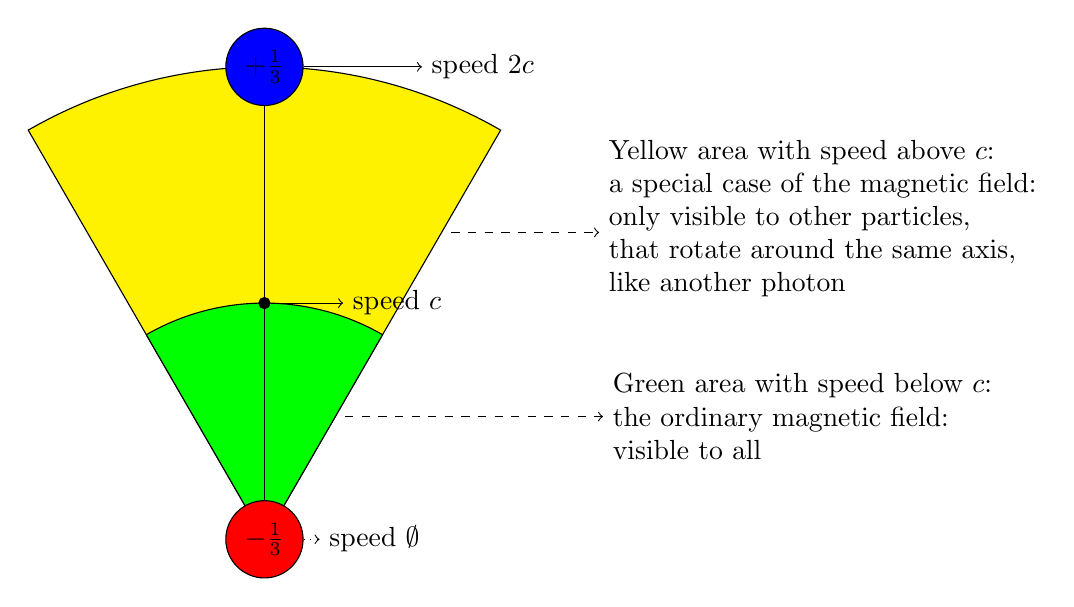
\begin{tikzpicture}[scale=1, rotate=0]

% photon vertical with green and yellow area for 
% sub and hyper c  indication speed 

\filldraw[fill=yellow, draw=black] (0,0) -- (60:6) 
node[pos=0.75, ](yellow) {} 
arc (60:120:6) -- (0,0);
\draw[->, dashed, black] (yellow) -- ++(2,0) node [right, align=left]
{Yellow area with speed above $c$: \\ 
a special case of the magnetic field: \\
only visible to other particles,  \\ 
that rotate around the same axis, \\
like another photon \\
};

\filldraw[fill=green, draw=black] (0,0) -- (60:3) 
node[pos=0.6, ](green) {} 
arc (60:120:3) -- (0,0);
\draw[->, dashed, black] (green) -- ++(3.4,0) node [right , align=left]
{
Green area with speed below $c$: \\ 
the ordinary magnetic field: \\ 
visible to all};


\path 
(0,0) node[circle,draw, fill=red]  (red) {$-\frac{1}{3}$}
(0,6) node[circle,draw, fill=blue] (blue) {$+\frac{1}{3}$};
\draw[black] (red) -- (blue)         node[pos=0.5](center){};
\filldraw
 (center) circle (2pt);
\draw[->, black] (center) -- ++(1,0) node [anchor=west]{speed $c$};
\draw[->, black] (blue) -- ++(2,0) node [anchor=west]{speed $2c$};
\draw[->, dotted] (red) -- ++(0.7,0) node [anchor=west]{speed $\emptyset$};

%\draw[->,dashed] (-5,4) to[out=60,in=180] (blue);



\end{tikzpicture}\caption{Photon vertical with green and yellow area for \\
 sub and hyper c  indication speed 
\label{fig:photon_green_yellow}}
\end{figure}
